\subsection{Теория рассеяния частиц}
\textbf{Постановка задачи.} Пусть из бесконечности летят легкие частицы, каждая массой $m$. В какой-то момент они пролетают мимо некоторой тяжелого тела массой $M$, испытывая воздействие с его стороны. Таким образом, изначально цилиндрический пучок частиц принимает коническую форму --- происходит рассеяние.\\

Классический пример этой задачи --- \href{https://en.wikipedia.org/wiki/Rutherford_scattering_experiments}{пример Резерфорда}.\\

\newpage

Еще один красивый пример --- \hyperref[grav_highway]{gravitational highway}.
\begin{figure}[!h]
    \centering
    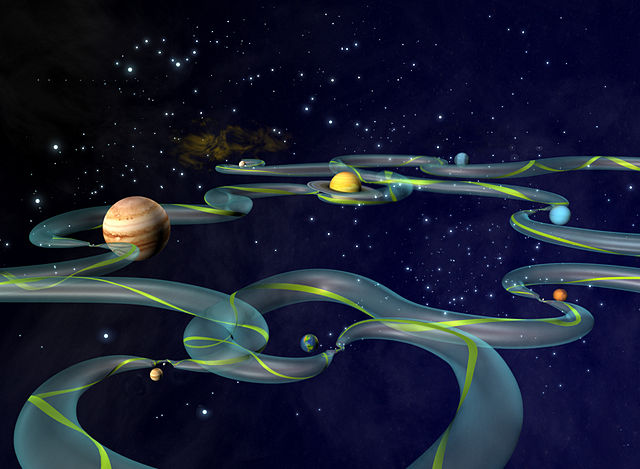
\includegraphics[width=0.5\linewidth]{images/лекция_8_1.jpg}
    \label{grav_highway}
\end{figure}

Вернемся к нашей задаче. Пусть $\rho$ --- прицельное расстояние, $\psi$ --- угол, на который отклоняется частица.
\begin{figure}[!h]
    \centering
    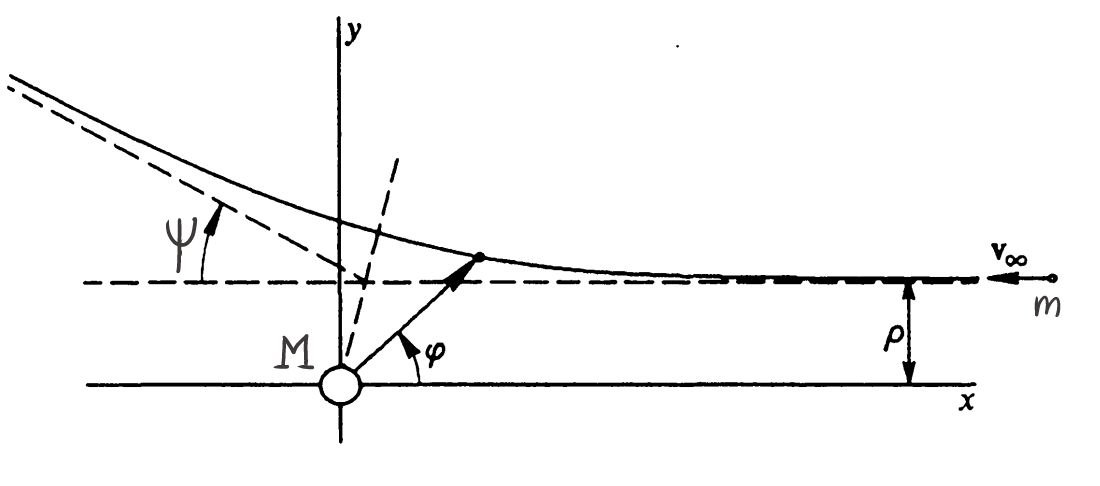
\includegraphics[width=0.75\linewidth]{images/лекция_8_2.jpeg}
\end{figure}
На частицу действует сила Кулона, тогда
\[
m \ddot{\vec{r}} = k \dfrac{e_1e_2}{\left(1 + \dfrac{m}{M}\right)^2} \cdot \dfrac{\vec{r}}{r^3} = \alpha \dfrac{\vec{r}}{r^3}
\]

Поле силы --- центральное. В полярной системе координат $\begin{pmatrix}
    x\\y\\
\end{pmatrix} = \begin{pmatrix}
    r\cos{\phi}\\r\sin{\phi}
\end{pmatrix}$
\[
m(\ddot{r} - r\dot{\phi}^2) = \dfrac{\alpha}{r^2}
\]
\[
\dfrac{d}{dt} (mr^2\dot{\phi}) = 0 \Longrightarrow K = const = mv_\infty\rho
\]
Сделав подстановку Бине, получим
\[
u'' + u = \dfrac{m\alpha}{K^2}
\]
Начальные условия: $u(0) = 0$, $u'(0) =\dfrac{1}{\rho}$. Получим решение в виде $u(\phi) = \dfrac{m\alpha}{K^2}(\cos{\phi} - 1) + \dfrac{1}{\rho}\sin{\phi}$, учитывая условие на K:
\[
u(\phi) = \dfrac{\alpha}{mv_\infty^2\rho^2}(\cos{\phi} - 1) + \dfrac{1}{\rho}\sin{\phi}
\]
Приравняем $u(\phi)$ к нулю, т.к. нужно получить угол, на котором частицы снова уйдут на бесконечность. Получим
\[
\rho = \dfrac{\alpha}{mv_\infty^2}\dfrac{1 - \cos{\phi}}{\sin{\phi}} = \dfrac{\alpha}{mv_\infty^2} ctg~\dfrac{\psi}{2}, \ \psi = \pi - \phi
\]
Пусть $d N$ --- число частиц, которые рассеиваются внутри угла от $\psi$ до $\psi + d \psi$, n --- число частиц, проходящих за единицу времени через единицу площади. Тогда \textbf{эффективное поперечное сечение рассеяния}:
\[
d \sigma = \dfrac{d N}{n}
\]
Если частицы вылетают из слоя от $\rho$ до $\rho + d\rho$, то они попадают в луч от $\psi$ до $\psi + d\psi$ $\Longrightarrow$
\[
dN = 2\pi\rho nd\rho \Longrightarrow d \sigma = \pi d\rho^2 = \pi \left(\dfrac{\alpha}{mv_\infty^2}\right)^2\dfrac{\cos{\psi / 2}}{\sin{\psi / 2}}d\psi = \pi \left(\dfrac{\alpha}{mv_\infty^2}\right)^2 d(ctg^2\psi/2)
\]

\section{Динамика твердого тела}
\subsection{Геометрия масс твердого тела}
\begin{reminder}
    Информация про \hyperlink{tenzor}{тензор инерции}.
\end{reminder}
\begin{wrapfigure}{l}{0.5\textwidth}
  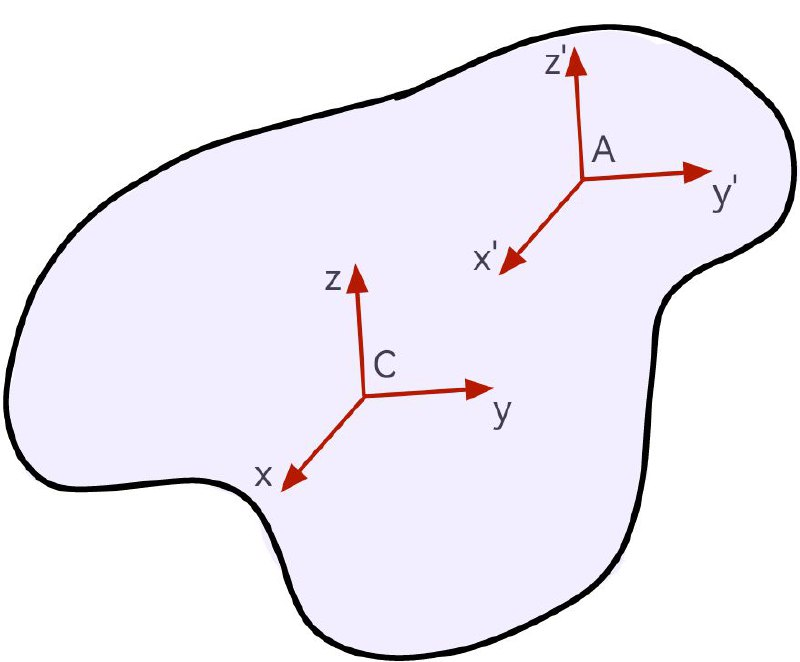
\includegraphics[width=0.8\linewidth]{images/лекция_8_3.jpeg}
\end{wrapfigure}
\tab\\
\begin{theorem}[Теорема Гюйгенса-Штейнера для тензора инерции]
    Пусть С --- центр масс тела, с ним связана система координат $xyz$, $A = (a,~b,~c)$ --- произвольная точка тела, заданная в осях центра масс, с ней связана система координат $x'y'z'$ такая, что $\begin{pmatrix}
        x'\\y'\\z'
    \end{pmatrix} = \begin{pmatrix}
        x - a\\y-b\\z - c\\
    \end{pmatrix}$, т.е. это параллельный перенос базиса из центра масс. В этом случае тензор инерции преобразуется по закону
    \[
    J_{A_{x'y'z'}} = J_{C_{xyz}} + m \cdot j_{C_{xyz}}(A)
    \]
    Т.е. момент инерции вокруг оси, проходящей через центр масс минимален.
\end{theorem}
\begin{proof}
    По определению момента инерции:
    \[
    J_{C_{xyz}} = \sum m_i \vec{r_i}^2 + 2\vec{d}\sum m_i \vec{r_i} + d^2 \sum m_i \tab J_{A_{x'y'z'}} = \sum m_i\vec{r_i}^2
    \]
    Здесь $\vec{r}_i$ --- положение точки в системе координат с началом в центре масс, $\vec{r'}_i$ --- в новой системе координат, $\vec{r'}_i = \vec{r}_i + \vec{d}$ ($\vec{d}$ --- вектор между старой и новой осями вращения). Тогда
    \[
    J_{A_{x'y'z'}} = \sum m_i \vec{r_i}^2 + 2\vec{d}\sum m_i \vec{r_i} + d^2 \sum m_i
    \]
    Т.к. в $C_{xyz}$ радиус-вектор центра масс равен нулю
    \[
    J_{A_{x'y'z'}} = \sum m_i \vec{r_i}^2 + d^2 \sum m_i
    \]
    Откуда следует искомая формула.
   
\end{proof}

В симметричных ситуациях вращение тела приобретает некоторые интересные свойства. Так, если 2 из 3 координат (a, b, c) равны нулю: если двигать оси вдоль одной из главных, то они так и останутся главными.

\begin{example}\end{example}
    \begin{minipage}{0.3\textwidth}% adapt widths of minipages to your needs
        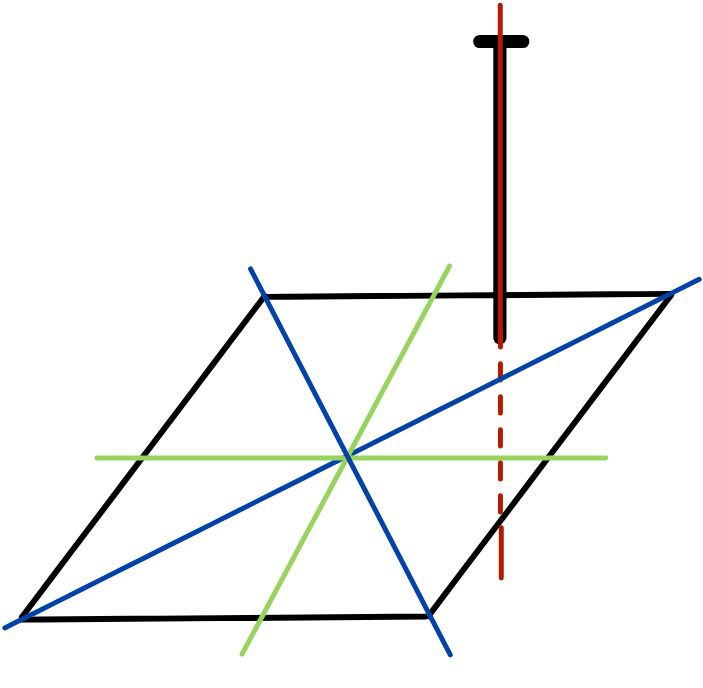
\includegraphics[width=1.0\textwidth]{images/лекция_8_4.jpeg} 
    \end{minipage}%
    \hfill%
    \begin{minipage}{0.6\textwidth}\raggedright
    Пусть имеется квадратная пластина, в которую воткнут гвоздь. Тогда одна из главных осей точно проходит вдоль гвоздя. А также любые две перпендикулярные друг другу в центре квадрата оси, лежащие в его плоскости, являются главными.
    \end{minipage}

\subsection{Эллипсоид инерции}
\begin{figure}[!h]
    \centering
    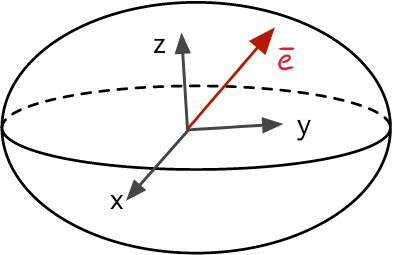
\includegraphics[width=0.3\linewidth]{images/лекция_8_5.jpeg}
\end{figure}
Пусть $\vec{e}$ --- произвольный орт. Во всех направлениях отложим $\dfrac{1}{\sqrt{J_{\vec{e}}}}$. Т.к. $J_{\vec{e}} = \vec{e}^TJ_{A_{xyz}}\vec{e}$, геометрическое место таких точек на концах векторов $\vec{u} = \dfrac{1}{\sqrt{J_{\vec{e}}}}\vec{e}$, то $\vec{u}^TJ_{A_{xyz}}\vec{u}$. Получим поверхность второго порядка
\[
Ax^2 + By^2 + Cz^2 + 2Dxy + 2Exz + 2Fyz = 1
\]
--- \textbf{эллипсоид инерции}, где А, В и С --- главные оси инерции.\\

\begin{frame}{Фан факт}
    На самом деле, эллипсоид инерции не всегда является эллипсоидом с геометрической точки зрения. Например для бесконечного стержня это цилиндр.
\end{frame}
\tab\\

Помним, что кинетический момент и кинетическую энергию можно найти как
\[
\vec{K}_A = J_{A_{xyz}}\vec{\omega} \tab \text{и} \tab T = \dfrac{1}{2}\vec{\omega}^TJ_{A_{xyz}}\vec{\omega}
\]
Тогда если тензор инерции задан в главных осях и $\vec{\omega} = \begin{pmatrix}p\\q\\r\\ \end{pmatrix}$ --- в проекции на оси, связанные с телом, то
\[
\vec{K}_A = \begin{pmatrix}
    Ap\\Bq\\Cr\\
\end{pmatrix} \tab \text{и} \tab T = \dfrac{1}{2}(Ap^2 + Bq^2 + Cr^2)
\]
Будем использовать этот результат в следующем разделе.\\



\subsection{Динамические уравнения вращательного движения тела}
Рассмотрим движение твердого тела с одной неподвижной точкой A, которую выберем в качестве полюса. В общем случае, когда нет закрепленной точки, результат, который будет получен далее, можно использовать, приняв за полюс центр масс, т.к. $\dot{\vec{K}}_C = \vec{M}_C^{out}$.\\

По теореме об изменении кинетического момента $\dot{\vec{K}}_A = \vec{M}_A^{out}$. Вектор угловой скорости задается в базисе $A_{xyz}$, связанном с телом. Т.к. тензор инерции относительно А в этом базисе не меняется
\[
\dot{K}_A = J_A\dot{\vec{\omega} + \vec{\omega}} \times J_A\vec{\omega} = \dfrac{\vec{K}_A}{d t} + \vec{\omega} \times \vec{K}_A
\]
Подставив покоординатную запись в теорему об изменении кинетического момента
\[
\begin{pmatrix}
    A\dot{p}\\B\dot{q}\\C\dot{r}\\
\end{pmatrix} + \begin{pmatrix}
    p\\q\\r\\
\end{pmatrix}\times\begin{pmatrix}
    Ap\\Bq\\Cr\\
\end{pmatrix} = \vec{M}_A^{O_{xyz}}
\]
 Раскрыв, получим \textbf{динамические уравнения Эйлера}:
 \[
 \begin{cases}
     A\dot{p} + (C - B) qr = M_A^x\\
     B\dot{q} + (A - C) pr = M_A^y\\
     C\dot{r} + (B - A) pq = M_A^z\\
 \end{cases}
 \]
 Здесь А, В и С --- главные оси инерции, $M_A^x$, $M_A^y$ и $M_A^z$ --- соответствующие проекции момента сил.\\

 Но этих уравнений недостаточно для решения задачи Коши. Нужно еще добавить \hyperlink{kinematic_Euler_equations}{кинематические уравнения Эйлера}, тогда интегрирование этой системы даст закон движения твердого тела в зависимости от сил и начальных условий.\\

 Можно доказать (но мы этого делать не будем), что динамические уравнения Эйлера --- неинтегрируемая система, но есть хорошие частные случаи. Известно три:
 \begin{enumerate}
     \item Случай Эйлера(-Пуансо)
     \item Случай Лагранжа(-Пуассона)
     \item Случай Ковалевской (не рассматривается в этом курсе)
 \end{enumerate}